\chapter{Foundations}
	\label{c:foundations}
	\IMRADlabel{methods}
	
	\section{Dynamical Systems}
		A \emph{dynamical system}~\cite{birkhoffDynamicalSystems1927} is a (physical) system that evolves over time \(t\) and is completely defined by the values of \(n\) real variables
		\begin{align*}
			x_1, x_2, \,\cdots\!, x_n \quad\longleftrightarrow\quad \vec{x} = \begin{bmatrix} x_1 & x_2 & \cdots & x_m \end{bmatrix}^T
		\end{align*}
		called the \emph{state} and often written in vector form (right). Given the differentiability of these values, we can also study their rate of change (often referred to as the "velocity") and the rate of change of the rate of change (often referred to as the "acceleration"):
		\begin{align*}
			\dot{\vec{x}} = \dv{\vec{x}}{t} \qquad \ddot{\vec{x}} = \dv[2]{\vec{x}}{t}
		\end{align*}
		Describing these systems is possible using differential equations, both ordinary and partial ones. A general \ac{ode} is given by an implicit equation
		\begin{align}
			\vec{0} = \vec{F}\big( \vec{x}, \vec{x}^{(1)}, \vec{x}^{(2)}, \,\cdots\!, \vec{x}^{(k - 1)}, \vec{x}^{(k)}; t \big),\quad \vec{x}^{(l)} \coloneqq \dv[l]{\vec{x}}{t}  \label{eq:ode}
		\end{align}
		which establishes a connection between the state itself and its time derivatives. We call a function \( \vec{x}(t) \) a \emph{solution} of an \ac{ode} if its derivatives fulfill the given \ac{ode}~\eqref{eq:ode}. We will now employ some definitions and terms that we will use throughout the whole thesis.
		\begin{description}[leftmargin = 3cm]
			\item[Order] If \( \vec{x}^{(k)} \) is the derivative of highest order that appears in the \ac{ode}, the \ac{ode} is called to be of order \(k\).
			\item[Linearity] An \ac{ode} is \emph{linear} if \(\vec{F}\) is a linear function in terms of the state and its derivatives, \ac{ie} it is given as a linear combination
		\end{description}
		\begin{align*}
			\vec{F} = \vec{r}(t) + \sum_{i = 1}^{k} c_i(t) \vec{x}^{(i)},\quad \vec{r}(t) : \R \to \R^n,\, c_i(t) : \R \to \R
		\end{align*}
		\begin{description}[leftmargin = 3cm]
			\item[Autonomous] If \(\vec{F}\) explicitly is independent of \(t\) (\ac{ie} \( \pdv{\vec{F}}{t} = \vec{0} \)), the \ac{ode} is called \emph{autonomous}.
			\item[Homogenity] If no term  of \(\vec{F}\) is independent of the state or its derivatives, the \ac{ode} is called \emph{homogeneous}. For any homogeneous \ac{ode} one of its solutions is the trivial solution \( \vec{x} \equiv \vec{0} \).
		\end{description}
		
		In all of the following, we assume to have explicit, autonomous, first order \acp{ode}. This is valid because we can transform every explicit higher order \ac{ode} into a system of first order \acp{ode} as well as we can introduce another "time state" which makes our \ac{ode} autonomous.
		
		The solution theory for linear \acp{ode} is highly evolved and solutions exist for nearly every possible \ac{ode}. But for nonlinear \acp{ode}, the world looks different. With the exception of some rare cases, nonlinear \acp{ode} are not tractable. Hence, we often need approximations for the nonlinear case. Some well-known approaches for these approximations are \ac{eg} \emph{small angle approximation} for Sines and Cosines. In small angle approximations, we Taylor-expand \( \sin \)/\( \cos \) and leave out all higher order terms:
		\begin{gather*}
			\sin(\varphi) = \varphi - \underbrace{\frac{\varphi^3}{3!} + \frac{\varphi^5}{5!} + \cdots}_\text{higher order terms} \approx \varphi \\
			\cos(\varphi) = 1 - \underbrace{\frac{\varphi^2}{2!} + \frac{\varphi^4}{4!} - \frac{\varphi^6}{6!} + \cdots}_\text{higher order terms} \approx 1
		\end{gather*}
		This approach is illustrated in~\autoref{fig:smallAngleApproximation}.
		
		\begin{figure}
			\centering
			\begin{subfigure}[t]{0.5\linewidth}
				\centering
				\includegraphics[width = \linewidth]{figures/introduction/generated/small-angle-approximation-sin.pdf}
				\caption{Small angle approximation \( \sin(\varphi) \approx \varphi \) of Sine.}
			\end{subfigure}%
			~
			\begin{subfigure}[t]{0.5\linewidth}
				\centering
				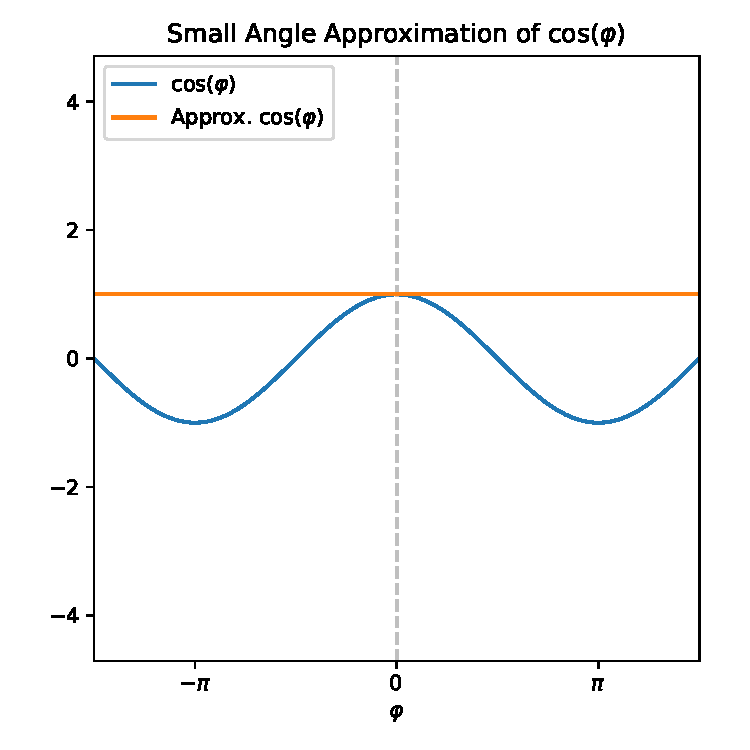
\includegraphics[width = \linewidth]{figures/introduction/generated/small-angle-approximation-cos.pdf}
				\caption{Small angle approximation \( \cos(\varphi) \approx 1 \) of Cosine.}
			\end{subfigure}
			\caption{Visualization of the small angle approximation (given is orange) of the basic trigonometric functions Sine and Cosine (given in blue). It is clear that the approximation is only valid in a small region around zero (\( \varphi \approx 0 \)).}
			\label{fig:smallAngleApproximation}
		\end{figure}
	
		We now look at two examples of dynamical systems, one which is linear and one that is not.
		
		\subsection{Harmonic Oscillator}
			\label{subsec:harmonicOscillator}
		
			\begin{figure}
				\centering
				\tikzHarmonicOscillator
				\caption{Illustration of a simple harmonic oscillator with mass \(m\), spring stiffness \(k\) and position \(x\) that is not affected by any external force like gravity. The mass is in equilibrium if \( x = 0 \).}
				\label{fig:simpleHarmonicOscillator}
			\end{figure}
	
			The \emph{simple harmonic oscillator} describes the dynamical system of a mass \(m\) that is attached to a spring that is following Hooke's Law with stiffness \(k\) (see~\autoref{fig:simpleHarmonicOscillator}). This harmonic oscillator is described by the \ac{ode}
			\begin{align}
				m\ddot{x} = -kx \quad\iff\quad \ddot{x} = -\frac{k}{m} x  \label{eq:harmonicOscillator}
			\end{align}
			where \(x\) and \(\ddot{x}\) are the position and acceleration of the mass, respectively. Note that if \( x = 0 \), the mass is in equilibrium and no force is acting on it.
			
			By using basic results in the solution theory of linear \acp{ode}, we see that the general solution is given as
			\begin{align*}
				x(t) = A \cos\Big(t \sqrt{k / m} + \varphi\Big)
			\end{align*}
			with the amplitude \(A\) and the phase \(\varphi\) (see~\autoref{app:harmonicOscillatorSolution} for the derivation of the solution). As neither gravity nor damping or other external forces are involved in the dynamical system, the motion continues forever with a non-changing amplitude.
		% end
		
		\subsection{Simple Pendulum}
			\label{subsec:simplePendulum}
			
			\begin{figure}
				\centering
				\tikzSimplePendulum
				\caption{Illustration of a simple pendulum with mass \(m\) and displacement \(\varphi\) that is only affected by gravity and no other external force. The mass is in equilibrium if \( \varphi = 0 \).}
				\label{fig:simplePendulum}
			\end{figure}
		
			The \emph{simple pendulum} described the dynamical system of a mass \(m\) that is attached to a rigid pole of length \(L\) which can freely swing around a suspension point (see~\autoref{fig:simplePendulum}). The motion of the pendulum is described by the \ac{ode}
			\begin{align*}
				\ddot{\varphi} = -\frac{g}{L} \sin(\varphi)
			\end{align*}
			where \(g\), \(L\), \(\varphi\) and \(\ddot{\varphi}\) describe the gravity acceleration, pole length, displacement and acceleration of the mass, respectively. Note that if \( \varphi = 0 \), the mass is in equilibrium and no force is acting on it.
			
			In comparison to the harmonic oscillator (\autoref{subsec:harmonicOscillator}), this differential equation is nonlinear. And, even for the case with unit gravity acceleration \( g = 1 \) and unit pole length \( L = 1\), where the \ac{ode} looks really simple
			\begin{align*}
				\ddot{\varphi} = -\sin(\varphi)
			\end{align*}
			it is not tractable analytically (\ac{ie} there exists no solution in closed form).
			
			Still, we can apply the small angle approximation introduced before (in this case, \( \sin(\varphi) \approx \varphi \)) which yields the \ac{ode} for a simple harmonic oscillator (see~\eqref{eq:harmonicOscillator}) with spring damping \( k = 1 \):
			\begin{align*}
				\ddot{\varphi} \approx -\varphi
			\end{align*}
			While this approximation forecasts movements around \( \varphi \approx 0 \) quite well\todo{be more scientific}, it fails for displacement far from zero.
			
			While this approximation works quite well for control problems like the cart pole, this approximation is only valid in a small region around \( \varphi \approx 0 \), where the system has a 
		% end
	% end
% end
